\subsection{Lagrange Approximation}

\frame{
\begin{itemize}
\item Interpolation means to estimate a missing function value by taking a weighted average of known function values at neighboring points. 
\item Linear interpolation uses a line segment that passes through two points. 
\end{itemize}
The slope between $(x_0, y_0)$ and $(x_1, y_1)$ is $m = (y_1 - y_0)/(x_1 - x_0)$, and the point-slope formula for the line $y = m(x - x_0) + y_0$ can be rearranged as 
\begin{equation*}
y = P(x) = y_0 + (y_1 - y_0) \frac{x - x_0}{x_1 - x_0}
\end{equation*}
When the above formula  is expanded, the result is a polynomial of degree $\le 1$. 
Evaluation of $P(x)$ at $x_0$ and $x_1$ produces $y_0$ and $y_1$, respectively: 
\begin{equation*}
\begin{array}{l c l c l}
P(x_0) & = & y_0 + (y_1 - y_0)(0) & = & y_0, \\
P(x_1) & = & y_0 + (y_1 - y_0)(1) & = & y_1.
\end{array}
\end{equation*}
}

\frame{
The French mathematician Joseph Louis Lagrange used a slightly different method to find this polynomial. 
He noticed that it could be written as 
\begin{equation*}
y = P_1(x) = y_0 \frac{x - x_1}{x_0 - x_1} + y_1 \frac{x - x_0}{x_1 - x_0}
\end{equation*}
Each term on the right side of (3.22) involves a linear factor; hence the sum is a polynomial of degree $\approx 1$. 
The quotients in (3.22) are denoted by 
\begin{equation*}
L_{1,0} (x) = \frac{x - x_1}{x_0 - x_1}
\ \ \ and \ \ \
L_{1,1} (x) = \frac{x - x_0}{x_1 - x_0}
\end{equation*}
Computation reveals that $L_{1,0}(x_0) = 1$, $L_{1,0}(x_1) = 0$, $L_{1,1}(x_0) = 0$, and $L_{1,1}(x_1) = 1$ so that the polynomial $P_1(x)$ in (3.22) also passes through the two given points: 
\begin{equation*}
P_1 (x_0) = y_0 + y_1(0) = y_0
\ \ \ and \ \ \
P_1 (x_1) = y_0(0) + y_1 = y_1.
\end{equation*}
}

\frame{
The terms $L_{1,0}(x)$ and $L_{1,1}(x)$ are called {\Large Lagrange coefficient polynomials} based on the nodes $x_0$ and $x-1$. 
Using this notation,  the summation form  can be written as
\begin{equation*}
P_1(x) = \sum_{k =0}^1 y_k L_{1,k} (x)
\end{equation*}
\begin{itemize}
\item Suppose that the ordinates $y_k$ are computed with the formula $y_k = f(x_k)$. 
\item If $P_1 (X)$ is used to approximate $f(x)$ over the interval $[x_0, x_1]$, we call the process {\Large interpolation}. 
\item If $x < x_0$ (or $x_1 < x$), then using $P_1 (x)$ is called {\Large extrapolation}. 
%\item The next example illustrates these concepts. 
\end{itemize}
}

\frame{
\frametitle{Example}
Consider the graph $y = f(x) = cos(x)$ over $[0.0,1.2]$. 
\begin{itemize}
\item (a) Use the nodes $x_0 = 0.0$ and $x_1 = 1.2$ to construct a linear interpolation polynomial $P_1(x)$. 
\item (b) Use the nodes $x_0 = 0.2$ and $x_1 = 1.0$ to construct a linear approximating polynomial $Q_1(x)$. 
\end{itemize}
\begin{center}
$\Downarrow$
\end{center}
Using  Lagrange polynomials with the abscissas $x_0 = 0.0$ and $x_1 = 1.2$ and the ordinates $y_0 = cos(0.0) = 1.000000$ and $y_1 = cos(1.2) = 0.362358$ produces
\begin{equation*}
\begin{array}{l c l}
P_1(x) & = & 1.000000 \frac{x - 1.2}{0.0 - 1.2} + 0.362358 \frac{x - 0.0}{1.2 - 0.0} \\
 & = & -0.833333(x - 1.2) + 0.301965(x - 0.0).
\end{array}
\end{equation*}
When the nodes $x_0 = 0.2$ and $x_1 = 1.0$ with $y_0 = cos(0.2) = 0.980067$ and $y_1 = cos(1.0) = 0.540302$ are used, 
the result is
\begin{equation*}
\begin{array}{l c l}
Q_1 (x) & = & 0.980067 \frac{x - 1.0}{0.2 - 1.0} + 0.540302 \frac{x - 0.2}{1.0 - 0.2} \\
 & = & -1.225083(x - 1.0) + 0.675378(x - 0.2).
\end{array}
\end{equation*}
}

\frame{
The following Figures (a) and (b) show the graph of $y = cos(x)$ and compare it with $y = P_1(x)$ and $y = Q_1(X)$, respectively. 
\begin{columns}
\begin{column}{0.5\textwidth}
\begin{figure}
\begin{center}
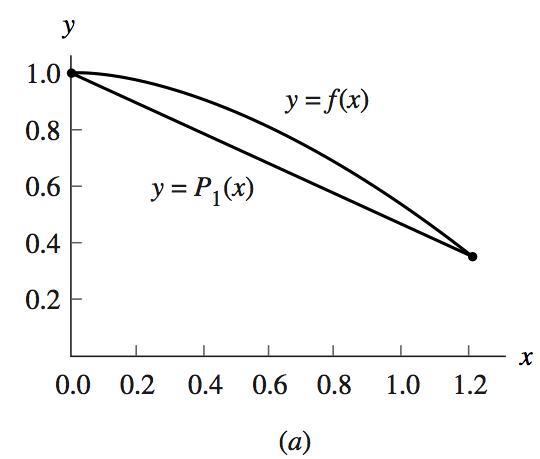
\includegraphics[width=50mm]{chap-3/fig_4-11.png}
\end{center}
\end{figure}
\end{column}
\begin{column}{0.5\textwidth}
\begin{figure}
\begin{center}
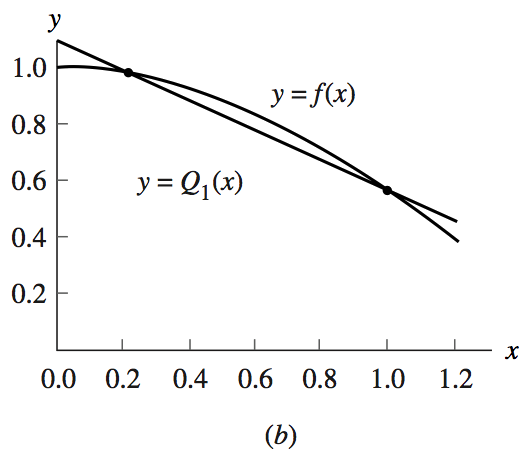
\includegraphics[width=50mm]{chap-3/fig_4-11_2.png}
\end{center}
\end{figure}
\end{column}
\end{columns}
}

\frame{
\begin{itemize}
\item Numerical computations are given in Table 3.6 and reveal that $Q_1(X)$ has less error at the points $x_k$ that satisfy $0.1 \le x_k \le 1.1$. 
\item The largest tabulated error, $f(0.6) - P_1(0.6) = 0.144157$, is reduced to $f(0.6) - Q_1(0.6) = 0.065151$ by using $Q_1(X)$. 
\end{itemize}
\begin{figure}
\begin{center}
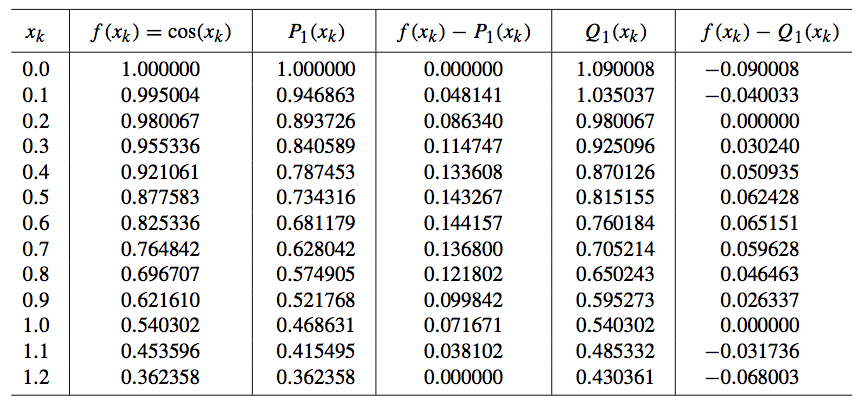
\includegraphics[width=90mm]{chap-3/tab_4-6.png}
\end{center}
\end{figure}
}

\frame{
The construction of a polynomial $P_N(X)$ of degree at most $N$ that passes through the $N + 1$ points $(x_0, y_0)$, $(x_1, y_1)$, $\ldots$, $(x_N, y_N)$ and has the form
\begin{equation*}
P_N (x) =\sum^N_{k=0} y_k L_{N,k} (x)
\end{equation*}
where $L_{N,k}$ is the Lagrange coefficient polynomial based on these nodes:
\begin{equation*}
L_{N,k} (x) = \frac{(x - x_0) \cdots (x - x_{k-1})(x - x_{k+1}) \cdots (x - x_N )}{(x_k - x_0) \cdots (x_k - x_{k-1})(x_k - x_{k+1}) \cdots (x_k - x_N )}
\end{equation*}
}





\frame{
It is understood that the terms $(x - x_k)$ and $(x_k - x_k)$ do not appear on the right side of equation (3.27). 
It is appropriate to introduce the product notation for (3.27), and we write 
\begin{equation*}
L_{N,k} (x) = \frac{\prod^N_{j=0, j\ne k} (x - x_j) }{\prod^N_{j=0, j\ne k} (x_k - x_j) } 
\end{equation*}
Here the notation in (3.28) indicates that in the numerator the product of the linear factors $(x - x_j)$ is to be formed, 
but the factor $(x - x_k)$ is to be left out (or skipped). 
A similar construction occurs in the denominator.
}

\frame{
A straightforward calculation shows that for each fixed $k$, the Lagrange coefficient polynomial $L_{N,k}(x)$ has the property 
\begin{equation*}
\begin{array}{l c l}
L_{N,k} (x_j ) = 1 \ \ when \ \  j = k 
\ \ \ and \ \ \  
L_{N,k} (x_j ) = 0 \ \ when \ \ j = k.
\end{array}
\end{equation*}
Then direct substitution of these values into (3.26) is used to show that the polynomial curve $y = P_N(x)$ goes through $(x_j,y_j)$:
\begin{equation*}
\begin{array}{l c l}
P_N ( x_j ) & = & y_0 L_{N,0} (x_j )+ \cdots + y_j L_{N, j} (x_j ) + \cdots + y_N L_{N,N} (x_j ) \\
& = & y_0(0) + \cdots + y_j (1) + \cdots + y_N (0) = y_j .
\end{array}
\end{equation*}
}

\frame{
\begin{itemize}
\item To show that $P_N(x)$ is unique, we invoke the fundamental theorem of algebra, which states that a nonzero polynomial $T(x)$ of degree $\le N$ has at most $N$ roots. 
\item In other words, if $T(x)$ is zero at $N + 1$ distinct abscissas, it is identically zero. 
\item Suppose that $P_N(x)$ is not unique and that there exists another polynomial $Q_N(x)$ of degree $\le N$ that also passes through the $N + 1$ points. 
\item Form the difference polynomial $T(x) = PN(x) - QN(X)$. 
\item Observe that the polynomial $T(x)$ has degree $\le N$ and that $T(x_j) = P_N(x_j) - Q_N(x_j) = y_j - y_j = 0$, for $j = 0,1,\ldots ,N$.
\item Therefore, $T(x) \equiv 0$ and it follows that $Q_N(x) = P_N(x)$.
\end{itemize}
}

\frame{
%When (3.26) is expanded, the result is similar to (3.22). 
The Lagrange quadratic interpolating polynomial through the three points $(x_0,y_0)$, $(x_1,y_1)$, and $(x_2,y_2)$ is
\begin{equation*}
P_2(x)
 = y_0 \frac{(x - x_1)(x - x_2)}{(x_0 - x_1)(x_0 - x_2)}
 + y_1 \frac{(x - x_0)(x - x_2)}{(x_1 - x_0)(x_1 - x_2)}
 + y_2 \frac{(x - x_0)(x - x_1)}{(x_2 - x_0)(x_2 - x_1)}
\end{equation*}
The Lagrange cubic interpolating polynomial through the four points $(x_0, y_0)$, $(x_1, y_1)$, $(x_2, y_2)$, and $(x_3, y_3)$ is 
\begin{equation*}
\begin{array}{l c l}
P_3(x) & = & y_0 \frac{(x - x_1)(x - x_2)(x - x_3)}{(x_0 - x_1)(x_0 - x_2)(x_0 - x_3)} + y_1 \frac{(x - x_0)(x - x_2)(x - x_3)}{(x_1 - x_0)(x_1 - x_2)(x_1 - x_3)} \\
 & = & + y_2 \frac{(x - x_0)(x - x_1)(x - x_3)}{(x_2 - x_0)(x_2 - x_1)(x_2 - x_3)} + y_3 \frac{(x - x_0)(x - x_1)(x - x_2)}{(x_3 - x_0)(x_3 - x_1)(x_3 - x_2)}
\end{array}
\end{equation*}
}

\frame{
\frametitle{Example }
Consider $y = f (x) = cos(x)$ over $[0.0, 1.2]$.
\begin{itemize}
\item (a) Use the three nodes $x_0 = 0.0$, $x_1 = 0.6$, and $x_2 = 1.2$ to construct a quadratic interpolation polynomial $P_2(x)$.
\item (b) Use the four nodes $x_0 = 0.0$, $x_1 = 0.4$, $x_2 = 0.8$, and $x_3 = 1.2$ to construct a cubic interpolation polynomial $P_3(x)$.
\end{itemize}
\begin{center}
$\Downarrow$
\end{center}
(a) Using $x_0 = 0.0$, $x_1 = 0.6$, $x_2 = 1.2$ and $y_0 = cos(0.0) = 1$, $y_1 = cos(0.6) = 0.825336$, and $y_2 = cos(1.2) = 0.362358$  produces
\begin{equation*}
\begin{array}{l c l}
P_2(x) & = & 1.0 \frac{(x - 0.6)(x - 1.2)}{(0.0 - 0.6)(0.0 - 1.2)} + 0.825336 \frac{(x - 0.0)(x - 1.2)}{(0.6 - 0.0)(0.6 - 1.2)} \\
 & & + 0.362358 \frac{(x - 0.0)(x - 0.6)}{(1.2 - 0.0)(1.2 - 0.6)} \\
& = & 1.388889(x - 0.6)(x - 1.2) - 2.292599(x - 0.0)(x - 1.2) \\
& & + 0.503275(x - 0.0)(x - 0.6).
\end{array}
\end{equation*}
}

\frame{
(b) Using $x_0 = 0.0$, $x_1 = 0.4$, $x_2 = 0.8$, $x_3 = 1.2$ and $y_0 = cos(0.0) = 1.0$, $y_1 = cos(0.4) = 0.921061$, $y_2 = cos(0.8) = 0.696707$, and $y_3 = cos(1.2) = 0.362358$ produces
\begin{equation*}
\begin{array}{l c l}
P_3(x) & = & 1.000000 \frac{(x - 0.4)(x - 0.8)(x - 1.2)}{(0.0 - 0.4)(0.0 - 0.8)(0.0 - 1.2)} \\
& & + 0.921061 \frac{(x - 0.0)(x - 0.8)(x - 1.2)}{(0.4 - 0.0)(0.4 - 0.8)(0.4 - 1.2)} \\ 
& & + 0.696707\frac{(x - 0.0)(x - 0.4)(x - 1.2)}{(0.8 - 0.0)(0.8 - 0.4)(0.8 - 1.2)} \\
& & + 0.362358 \frac{(x - 0.0)(x - 0.4)(x - 0.8)}{(1.2 - 0.0)(1.2 - 0.4)(1.2 - 0.8)} \\
& = & -2.604167(x - 0.4)(x - 0.8)(x - 1.2) \\
& & + 7.195789(x - 0.0)(x - 0.8)(x - 1.2) \\
& & - 5.443021(x - 0.0)(x - 0.4)(x - 1.2) \\
& & + 0.943641(x - 0.0)(x - 0.4)(x - 0.8).
\end{array}
\end{equation*}
}



\frame{
The graphs of $y = cos(x)$ and the polynomials $y = P_2(x)$ and $y = P_3(x)$ are shown in Figure 3.12(a) and (b), respectively. 
\begin{columns}
\begin{column}{0.5\textwidth}
\begin{figure}
\begin{center}
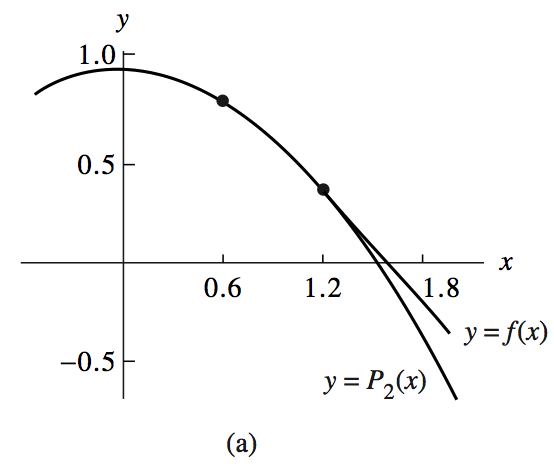
\includegraphics[width=50mm]{chap-3/fig_4-12.png}
\end{center}
\end{figure}
\end{column}
\begin{column}{0.5\textwidth}
\begin{figure}
\begin{center}
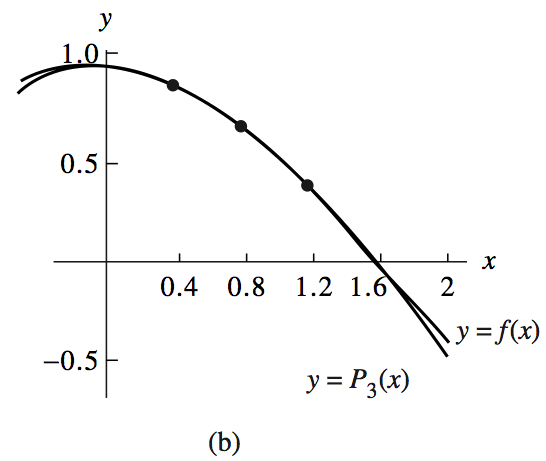
\includegraphics[width=50mm]{chap-3/fig_4-12_2.png}
\end{center}
\end{figure}
\end{column}
\end{columns}
}

\frame{
\frametitle{Error Terms and Error Bounds}
\begin{itemize}
\item It is important to understand the nature of the error term when the Lagrange polynomial is used to approximate a continuous function $f(x)$. 
\item It is similar to the error term for the Taylor polynomial, except that the factor $(x-x_0)^{N+l}$ is replaced with the product $(x - x_0)(x - x_1)\cdots(x - x_N)$. 
\item This is expected because interpolation is exact at each of the $N + 1$ nodes $x_k$, where we have $E_N(x_k) = f(x_k) - P_N(x_k) = y_k -y_k = 0$ for $k = 0, 1, 2, \ldots, N$. 
\end{itemize}
}

\frame{
\begin{block}{Theorem (Lagrange Polynomial Approximation). }
Assume that $f \in C^{N+1}[a, b]$ and that $x_0$, $x_1$, $\ldots$, $x_N \in [a, b]$ are $N + 1$ nodes. 
If $x \in [a, b]$, then
\begin{equation*}
f (x) = P_N (x) + E_N (x),
\end{equation*}
where $P_N (x)$ is a polynomial that can be used to approximate $f (x)$:
\begin{equation*}
f (x) \approx P_N (x) = \sum^N_{k=0} f (x_k)L_{N,k} (x).
\end{equation*}
The error term $E_N (x)$ has the form
\begin{equation*}
E_N (x) = \frac{(x - x_0)(x - x_1) \cdots (x - x_N ) f^{(N+1)}(c)}{(N + 1)!}
\end{equation*}
for some value $c = c(x)$ that lies in the interval $[a, b]$.
\end{block}
}

\frame{
\frametitle{Proof of Theorem }
As an example of the general method, we establish (3.35) when $N = 1$. 
 The general case is discussed in the exercises. 
Start by defining the special function $g(t)$ as 
\begin{equation*}
g(t) = f (t) - P_1(t) - E_1(x) \frac{(t - x_0)(t - x_1)}{(x - x_0)(x - x_1)}
\end{equation*}
Notice that $x$, $x_0$, and $x_1$ are constants with respect to the variable t and that $g(t)$ evaluates to be zero at these three values; that is,
\begin{equation*}
g(x) = f (x) - P_1(x) - E_1(x) \frac{(x - x_0)(x - x_1)}{(x - x_0)(x - x_1)} = f (x) - P_1(x) - E_1(x) = 0,
\end{equation*}
\begin{equation*}
g(x_0) = f (x_0) - P_1(x_0) - E_1(x) \frac{(x_0 - x_0)(x_0 - x_1)}{(x - x_0)(x - x_1)} = f (x_0) - P_1(x_0) = 0,
\end{equation*}
\begin{equation*}
g(x_1) = f (x_1) - P_1(x_1) - E_1(x) \frac{(x_1 - x_0)(x_1 - x_1)}{(x - x_0)(x - x_1)} = f (x_1) - P_1 (x_1) = 0
\end{equation*}
}

\frame{
Suppose that $x$ lies in the open interval $(x_0, x_1)$. 
Applying Rolle’s theorem to $g(t)$ on the interval $[x_0, x]$ produces a value $d_0$, with $x_0 < d_0 < x$, such that
\begin{equation*}
g'(d_0) = 0
\end{equation*}
A second application of Rolle’s theorem to $g(t)$ on $[x, x_1]$ will produce a value $d_1$, with $x < d_1 < x_1$, such that
\begin{equation*}
g'(d_1) = 0
\end{equation*}
So the function $g'(t)$ is zero at $t = d_0$ and $t = d_1$. \\
A third use of Rolle’s theorem, but this time applied to $g'(t)$ over $[d_0, d_1]$, produces a value c for which
\begin{equation*}
g^{(2)}(c) = 0
\end{equation*}
}

\frame{
Now  compute the derivatives $g'(t)$ and $g^{(2)}(t)$:
\begin{equation*}
g'(t) = f'(t) - P_1'(t) - E_1'(x) \frac{(t - x_0) + (t - x_1)}{(x - x_0)(x - x_1)}
\end{equation*}
\begin{equation*}
g^{(2)}(t) = f^{(2)}(t) - 0 - E_1(x)\frac{2}{(x - x_0)(x - x_1)}
\end{equation*}
we have used the fact the $P_1(t)$ is a polynomial of degree $N = 1$; 
hence its second derivative is $P_1^{(2)}(t) ≡ 0$. 
Evaluation  at the point $t = c$ 
\begin{equation*}
0 = f^{(2)}(c) - E_1(x) \frac{2}{(x - x_0)(x - x_1)}
\end{equation*}
Solving $E_1(x)$ results in the desired form for the remainder:
\begin{equation*}
E_1(x) =\frac{(x - x_0)(x - x_1) f^{(2)}(c)}{2!}
\end{equation*}
}

\frame{
The next result addresses the special case when the nodes for the Lagrange polynomial are equally spaced $x_k = x_0 + hk$, for $k = 0$, $1$, $\ldots$, $N$, and the polynomial $P_N(x)$ is used only for interpolation inside the interval $[x_0, x_N]$.
}

\frame{
\begin{block}{Theorem (Error Bounds for Lagrange Interpolation, Equally Spaced Nodes).}
Assume that $f(x)$ is defined on $[a, b]$, which contains equally spaced nodes $x_k = x_0 + hk$. 
Additionally, assume that$ f(x)$ and the derivatives of $f(x)$, up to the order $N + 1$, are continuous and bounded on the special subintervals $[x_0, x_1]$, $[x_0, x_2]$, and $[x_0, x_3]$, respectively; that is,
\begin{equation*}
\left| f^{(N+1)} (x) \right| \le M_{N+1} \ \ \  for \ \ \ x_0 \le x \le x_N ,
\end{equation*}
for $N = 1, 2, 3$. 
The error terms corresponding to the cases $N = 1$, $2$, and $3$ have the following useful bounds on their magnitude:
\begin{equation*}
\begin{array}{l c c l}
\left| E_1(x) \right| \le \frac{h^2 M_2}{8} &  valid & for & x \le [x_0, x_1], \\
\left| E_2(x) \right| \le \frac{h^3 M_3}{9} &  valid & for & x \le [x_0, x_2], \\
\left| E_3(x) \right| \le \frac{h^4 M_4}{24} &  valid & for & x \le [x_0, x_3],
\end{array}
\end{equation*}
\end{block}
}

\frame{
\frametitle{Proof of Theorem }
Using the change of variables $x - x_0 = t$ and $x - x_1 = t - h$, the error term $E_1(x)$ can be written as
\begin{equation*}
E_1(x) = E_1( x_0 + t) =\frac{(t^2 - ht) f^{(2)} (c)}{2!} \ \ \ for \ \ 0 \le t \le h.
\end{equation*}
The bound for the derivative for this case is
\begin{equation*}
\left| f^{(2)} (c) \right| \le M_2 \ \ \  for x_0 \le c \le x_1
\end{equation*}
Now determine a bound for the expression $(t^2 - ht)$;  call this term $\phi (t) = t_2- ht$.
Since $\phi'(t) = 2t - h$, there is one critical point $ t = h \slash 2$ that is the solution to $\phi'(t) = 0$.
The extreme values of $\phi(t)$ over $[0, h]$ occur either at an end point $\phi(0) = 0$, $\phi(h) = 0$ or at the critical point $\phi(h/2) = - h^2 \slash 4$. 
}

\frame{
Since the latter value is the largest, we have established the bound
\begin{equation*}
\left| \phi (t) \right| = \left| t^2 - ht \right| \le \frac{\left| -h^2 \right|}{4} = \frac{h^2}{4} \ \ \ for \ \ 0 \le t \le h
\end{equation*}
\begin{center}
$\Downarrow$
\end{center}
\begin{equation*}
\left| E_1(x) \right| = \frac{\left| \phi(t) \right| \left| f^{(2)}(c)\right| }{2!} \le \frac{h^2 M_2}{8}
\end{equation*}
and formula of theorem  is established.
}











